\subsection{Overview}

As explained in the RASD and DD documents, the system requires the following components to be fully developed and working:
\begin{itemize}
	\item \textbf{Travlendar+ mobile application, working on Android v 4.0.3 and later;}
	\item \textbf{JBoss 7.0.1 Java Server, running the Travlendar+ application services;}
	\item \textbf{MySQL 5.7.19 DBMS for users data managing;}
\end{itemize}
Furthermore, the Travlendar+ application services component is composed by the following subsystems, wich must be developed and correctly integrated:
\begin{itemize}
	\item \textbf{Appointment manager}, which makes use of Calendar APIs and requires DBMS connection;
	\item \textbf{Travel manager}, which implements Weather and Maps APIs;
	\item \textbf{Account manager},
	\item \textbf{Tickets manager},
\end{itemize}
Finally, the following connection must be implemented and full working:
\begin{itemize}
	\item \textbf{Remote Method Invocation} connection between client and application server, using JRMP protocol;
	\item \textbf{JDBC} connection between application server and DBMS.
\end{itemize}

\subsection{Strategy}
In order to guarantee observability and efficacy, the testing strategy follows an incremental integration logic. The chosen approach is bottom-up: this choice allows us to gradually build the system and continuously provide feedbacks as soon as the single parts are finished. Our goal is to first develop sub-component that are able to work independently and do not require connections with other parts of the systems. Then, once that all sub-components are fully developed and tested, we plan to proceed in connecting them and fulfill the dependencies to implement gradually the main super-component functions. Final part of the integration will require the main component to be full working and tested, and consists in testing the correct working of connections between main-components. 

\subsection{Dependecies}
The interaction with DBMS is essential for the correct working of all the four main components of the Application services. Plus, Appointment Manager requires Account Manager to be implemented to ensure the correctness of the links between different accounts and relative calendars:

\begin{figure}[H]
	\centering
	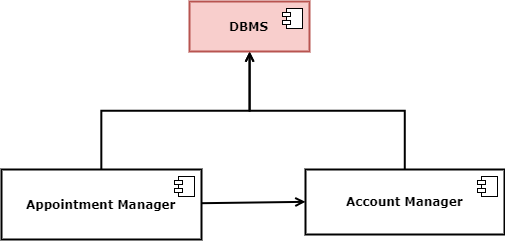
\includegraphics[width=0.5\textwidth]{Images/Test/1.png}%
\end{figure}

In order to work properly, Travel Manager makes use of different external APIs such as Maps APIs, Weather APIs and different APIs from car sharing and bike sharing services. The correct functionality of these interfaces must be checked before proceeding in developing the component. In addition, Travel Manager requires an integration with Appointment Manager to acquire data relative to the different locations of the appointments.

\begin{figure}[!h]
	\centering
	\makebox[\textwidth][c]{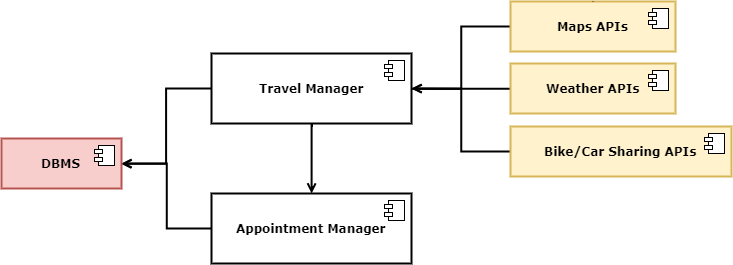
\includegraphics[width=0.5\textwidth]{Images/Test/2.png}}%
\end{figure}

Finally, Tickets Manager strictly depends on the correct working of the APIs of the chosen ticket provider to pay and acquire travel tickets. It also requires Travel Manager to work properly, because the user can accesstickets functionalities only after selecting a movement from the daily schedule. 

\begin{figure}[!h]
	\centering
	\makebox[\textwidth][c]{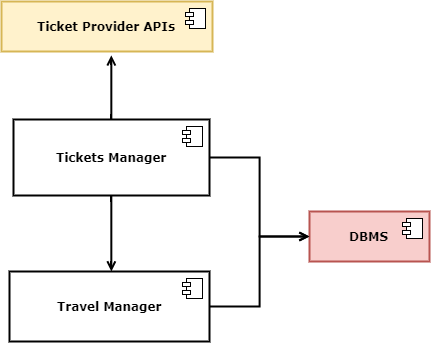
\includegraphics[width=0.5\textwidth]{Images/Test/3.png}}%
\end{figure}


Given the previous information, an appropriate plan of integration and testing could be the following one:\\
\textbf{Week 27/11/17 – 4/12/17:}
\begin{itemize}
	\item DBMS: build a simple Java application that interacts with MySQL 5.7.19 Database Manage System by JDBC and correctly store and manage data from a small database.
	\item ACCOUNT MANAGER: expand the application, allowing different users to register and insert personal info. 
	\item MAPS APIs: testing APIs with small example applications to ensure correct working.
	\item WEATHER APIs: testing APIs with small example applications to ensure correct working.
\end{itemize}
\textbf{Week 4/12/17 – 18/12/17:}
\begin{itemize}
	\item CAR/BIKE SHARING APIs: testing APIs with small example applications to ensure correct working.
	\item ACCOUNT MANAGER: fully development and testing of all component functionalities: allow multiple users to register and login, manage personal data and connect existing Facebook/Google account.
	\item APPOINTMENT MANAGER: expand the application by giving the user the possibility of creating, editing and delete simple appointments (no alert/advanced option). Test the correct storage in the database and the correct integration with Account Manager.
	\item start working on network platform: develop a small application that makes use of RMI technology to invoke methods on an example application running on JBoss 7.0.1 Java Server.
\end{itemize}
\textbf{Week 4/12/17 – 18/12/17:}
\begin{itemize}
	\item APPOINTMENT MANAGER: fully development and testing of all component functionalities: allow the user to add advanced options to the different appointments. Test full integration with Account Manager.
	\item TRAVEL MANAGER: integrate use of Maps/Weather/Car\&Bike Sharing APIs with data provided by Appointment Manager to compute travels for each appointment. Testing of the functionalities.
	\item TICKET PROVIDER APIs: testing APIs with small example applications to ensure correct working.
	\item Export the application on JBoss 7.0.1 Java Server, testing of RMI methods to access the application features from remote.
\end{itemize}
\textbf{Week 18/12/17 – 8/1/18:}
\begin{itemize}
	\item TRAVEL MANAGER: fully development and testing of all component functionalities: the application accesses correctly appointment and user data to compute travels. Test complete integration with Appointment Manager.
	\item TICKET MANAGER: expand the application by adding functionalities for tickets purchase using the tested APIs. Test integration with Travel Manager.
\end{itemize}
\textbf{Week 8/1/18– 18/1/18:}
\begin{itemize}
	\item General testing of full application functionalities.
\end{itemize}